
\section{Medições em laboratório}


Montaremos os dois circuitos discutidos acima em laboratório, e mediremos a tensão de entrada e saída para várias frequências, e com isto obteremos a magnitude da função transferência para frequências diversas.


\begin{figure}[h]
    \centering
    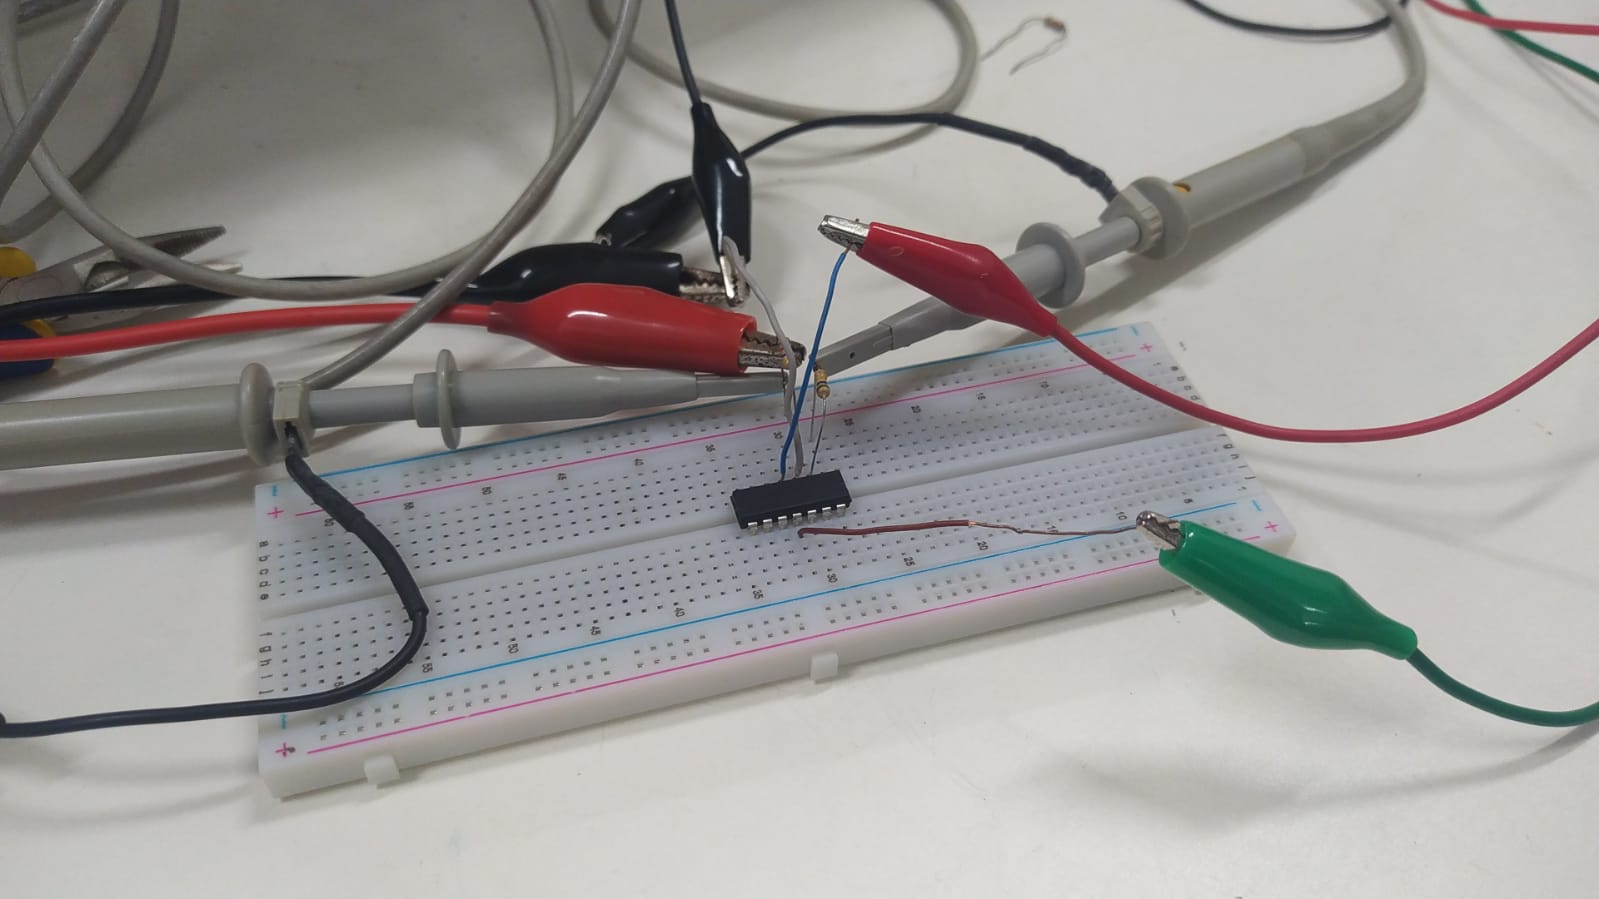
\includegraphics[width=1\columnwidth]{images/circuitoreal.jpeg}
    \caption{Foto do circuito montado em laboratório.}
\end{figure}


\subsection{Circuito 1}


\subsubsection{Valores dos componentes}


\begin{equation}
    \begin{aligned}
        R_1 = 4.65k \varOmega \\
        R_2 = 21.9k \varOmega \\
    \end{aligned}
\end{equation}


\subsubsection{Frequência de corte}


Identificamos a frequência de corte como sendo $f_c = 210 kHz$.


\subsubsection{Valores medidos}


\begin{figure}[H]
    \centering
    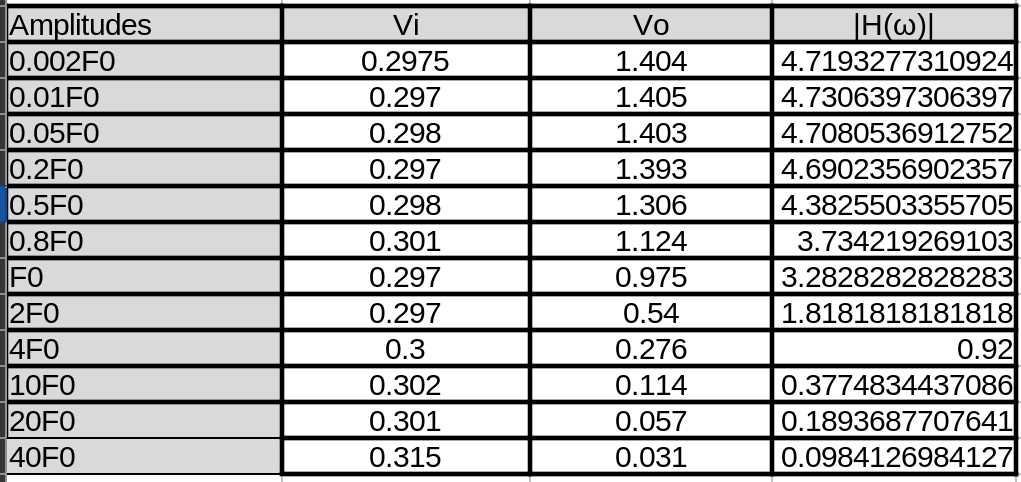
\includegraphics[width=1\columnwidth]{images/valores1.png}
    \caption{Tabela de magnitude para uma gama de valores de frequência.}
\end{figure}


\subsubsection{Fotos do osciloscópio}


\begin{figure}[H]
    \centering
    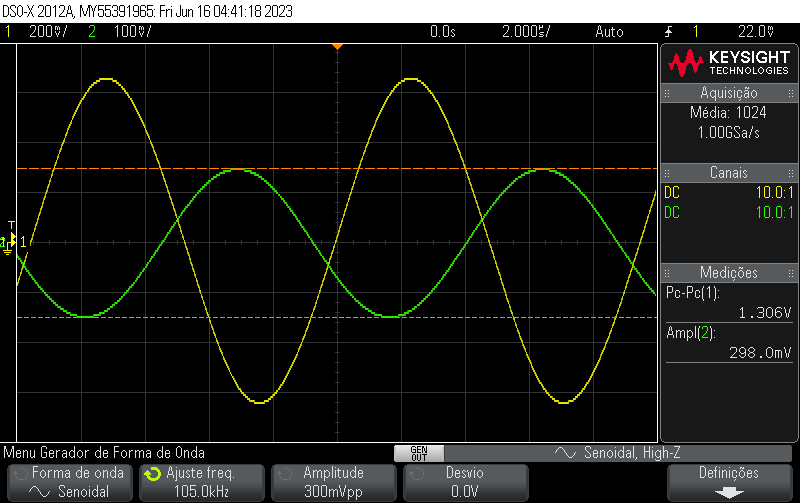
\includegraphics[width=1\columnwidth]{images/exemplo1_meio_fc.png}
    \caption{Imagem da onda no osciloscópio para 0.5 $f_c$.}
\end{figure}


\begin{figure}[H]
    \centering
    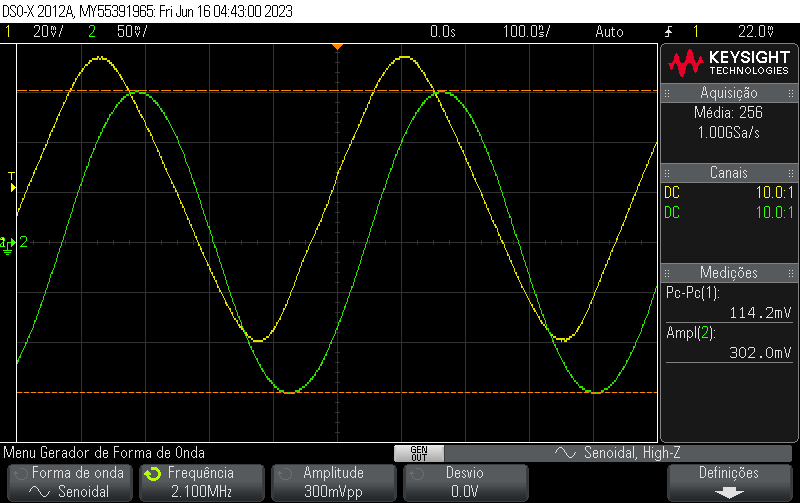
\includegraphics[width=1\columnwidth]{images/exemplo1_10_fc.png}
    \caption{Imagem da onda no osciloscópio para 10 $f_c$.}
\end{figure}


\begin{figure}[H]
    \centering
    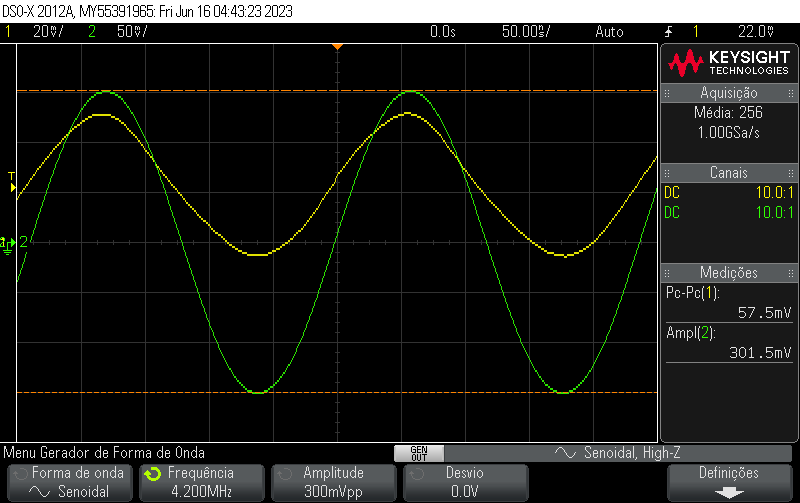
\includegraphics[width=1\columnwidth]{images/exemplo1_20_fc.png}
    \caption{Imagem da onda no osciloscópio para 20 $f_c$.}
\end{figure}
\newpage


\subsection{Circuito 2}


\subsubsection{Valores dos componentes}


\begin{equation}
    \begin{aligned}
        R_1 = 4.65k \varOmega \\
        R_2 = 550k \varOmega  \\
    \end{aligned}
\end{equation}


\subsubsection{Frequência de corte}


Identificamos a frequência de corte como sendo $f_c = 11800 kHz$.


\subsubsection{Valores medidos}


\begin{figure}[h]
    \centering
    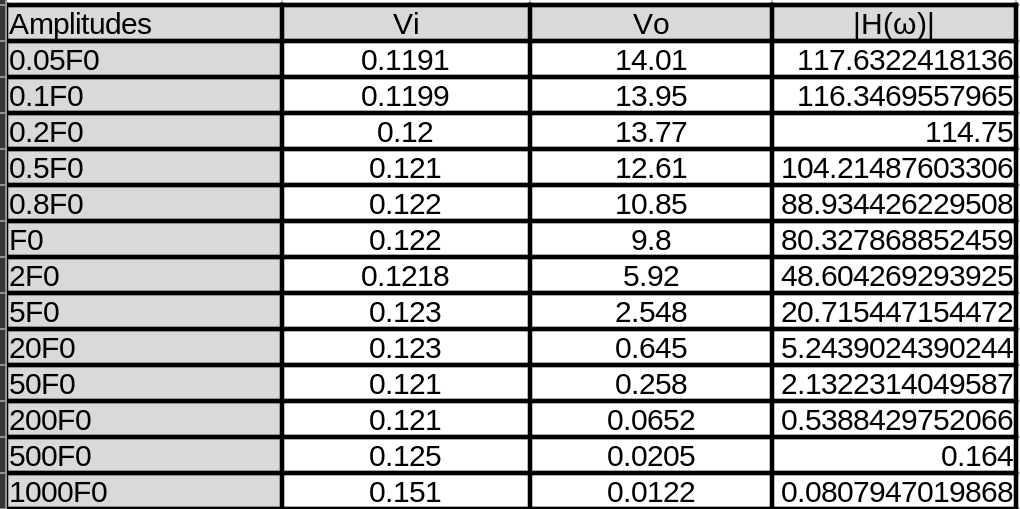
\includegraphics[width=1\columnwidth]{images/valores2.png}
    \caption{Tabela de magnitude para uma gama de valores de frequência.}
\end{figure}


\subsubsection{Fotos do osciloscópio}


\begin{figure}[h]
    \centering
    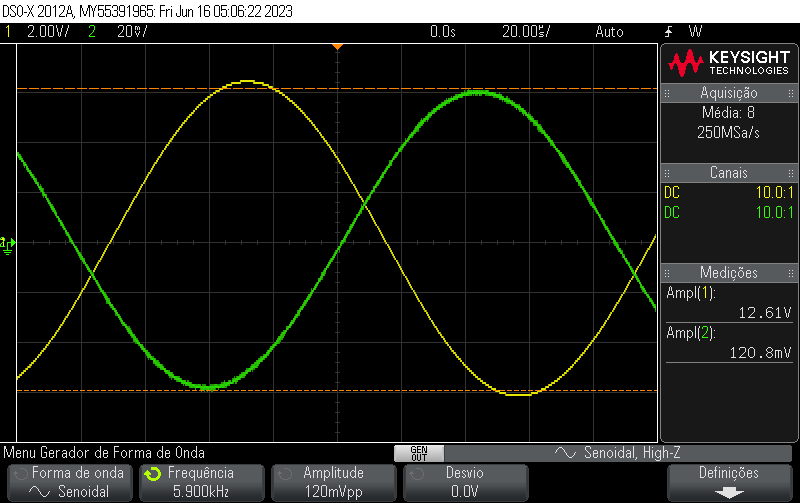
\includegraphics[width=1\columnwidth]{images/exemplo2_meio_fc.png}
    \caption{Imagem da onda no osciloscópio para 0.5 $f_c$.}
\end{figure}


\begin{figure}[h]
    \centering
    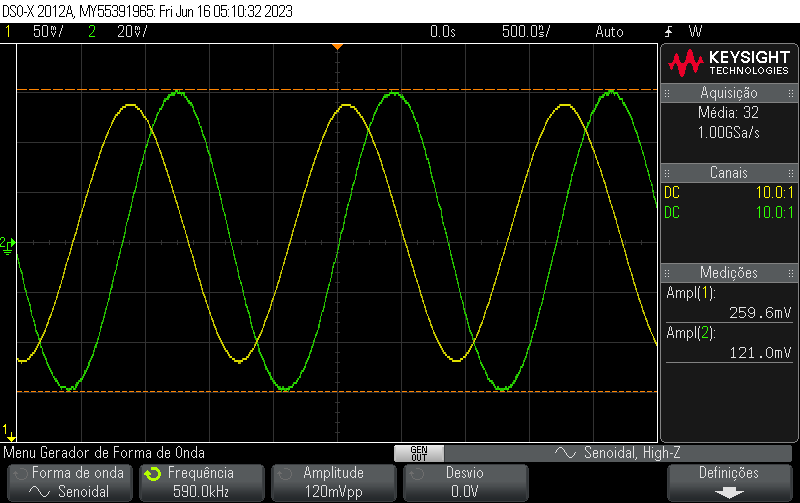
\includegraphics[width=1\columnwidth]{images/exemplo2_50_fc.png}
    \caption{Imagem da onda no osciloscópio para 50 $f_c$.}
\end{figure}


\begin{figure}[h]
    \centering
    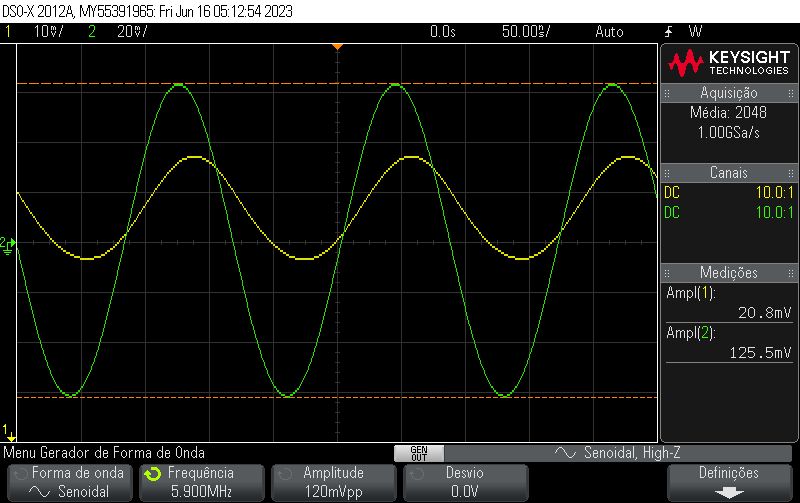
\includegraphics[width=1\columnwidth]{images/exemplo2_500_fc.png}
    \caption{Imagem da onda no osciloscópio para 500 $f_c$.}
\end{figure}


\newpage
